\subsubsection{Exascale MPI} \label{subsubsect:mpich}
\paragraph{Overview}

MPI has been the de facto standard programming model for HPC from the
mid 90's till today, a period where supercomputing performance
increased by six orders of magnitude.  The vast majority of DOE's
parallel scientific applications running on the largest HPC systems
use MPI.  These application codes represent billions of dollars of
investment.  Therefore, MPI must evolve to run as efficiently as
possible on Exascale systems.  Our group at Argonne developed a
high-performance, production-quality MPI implementation, called MPICH.
The focus areas of the Exascale MPI / MPICH project are: (1)
continuous improvement of the performance and capabilities of the
MPICH software to meet the demands of ECP and other broader DOE
applications, (2) coordinate vendor and supercomputing center
interactions to ensure efficient solutions to applications, and (3) be
involved in the MPI forum and standardization efforts to ensure
continuity of the work beyond this project.


\paragraph{Key  Challenges}

While we believe MPI is a viable programming model at Exascale, both
the MPI standard and MPI implementations have to address the
challenges posed by the increased scale, performance characteristics
and evolving architectural features expected in Exascale systems, as
well as the capabilities and requirements of applications targeted at
these systems.  The key challenges are:

\begin{enumerate}

\item Interoperability with intranode programming models having a high
  thread count \cite{Hybrid1, Hybrid2, FT2} (such as OpenMP,
  OpenACC and emerging asynchronous task models);

\item Scalability and performance over complex architectures
  \cite{Perf1, Perf2, FT2, Perf4} (including high core counts,
  processor heterogeneity and heterogeneous memory);

\item Software overheads that are exacerbated by lightweight cores and
  low-latency networks;

\item Enhanced functionality (extensions to the MPI standard) based on
  experience with applications and high-level libraries/frameworks
  targeted at Exascale; and

\item Topics that become more significant as we move to the next
  generation of HPC architectures: memory usage, power, and
  resilience.

\end{enumerate}


\paragraph{Solution Strategy}

The Exascale MPI project has the following primary technical thrusts:
(1) \textbf{Performance and Scalability} (2) \textbf{Heterogeneity}
(3) \textbf{Topology Awareness} (4) \textbf{Fault Tolerance} and (5)
\textbf{MPI+X Hybrid Programming}.

Our solution strategy started by addressing performance and
scalability aspects in MPICH related to network address management
\cite{memscal}.  Apart from this, we also looked at communication
strategies which allow the MPI library to be as lightweight as
possible \cite{ch41, ch42}.  Other ongoing solutions include
investigation and evaluation of communication relaxation hints,
investigation of optimizations to memory scalability in MPICH and
improvements to MPI RMA operations.

Exascale MPI heterogeneity efforts \cite{Hetero1, Hetero2, Hetero3}
started with the survey on heterogeneous memory architectures on
upcoming DOE machines and how MPICH can take advantage of them
\cite{hexe}.  The ongoing efforts include the investigation of
utilizing heterogeneous memory inside the MPI implementation and
evaluation of applications.

Exascale MPI topology awareness efforts \cite{Topo1,Topo2} originated
with the investigation and evaluation of hints based on topology
awareness and optimizations to virtual topology functionality in MPICH
\cite{topo-io,topo-io2}.  The ongoing efforts include investigation of
topology-aware collectives and neighborhood collectives in MPICH
\cite{coll} and evaluation of the selected ECP applications.

Exascale MPI fault tolerance efforts \cite{FT1, FT2} started with
support for handling noncatastrophic errors in MPI.  The second effort
included defining the scope of errors in MPI, a prerequisite for
user-level failure mitigation (ULFM).  Other efforts that we are
looking at in this direction are standardizing ULFM in MPI and
evaluating application suitability for fault tolerance.

Exascale MPI+X hybrid programming developed firstly with effort in
improving interoperation of MPICH with threads \cite{interthread}.
Secondly, we included support for interaction of MPICH with user-level
thread (ULT) libraries \cite{ULT}, primarily targeting Argobots and
the BOLT runtime and the work-queue data transfer model for
multithreaded MPI communication.  Other issues that are being looked
at include the investigation and evaluation on interaction between MPI
and OpenMP and the study and evaluation of MPI endpoints.


\paragraph{Recent Progress}

Figure~\ref{fig:march18} provides the details of the milestones
completed in FY18Q1 and FY18Q2.  Milestones completed in December 2017
include: (1) classifying what noncatastrophic errors; when
noncatastrophic errors occur (e.g., upon exhaustion of resources), our
implementation informs the user of the error without disrupting MPI
functionality.  (2) topology-aware communicator split for NUMA, cache,
and other on-node hardware resources, as well as for storage systems
\cite{topo-io,topo-io2}, such that the newly created communicators are
local to processes sharing hardware resources.  (3) error scope
definition as a prerequisite for user-level failure mitigation; we
clarified how errors should be handled when they are not attached to a
communicator, window, or file.

\begin{figure}[htb]
  \centering
  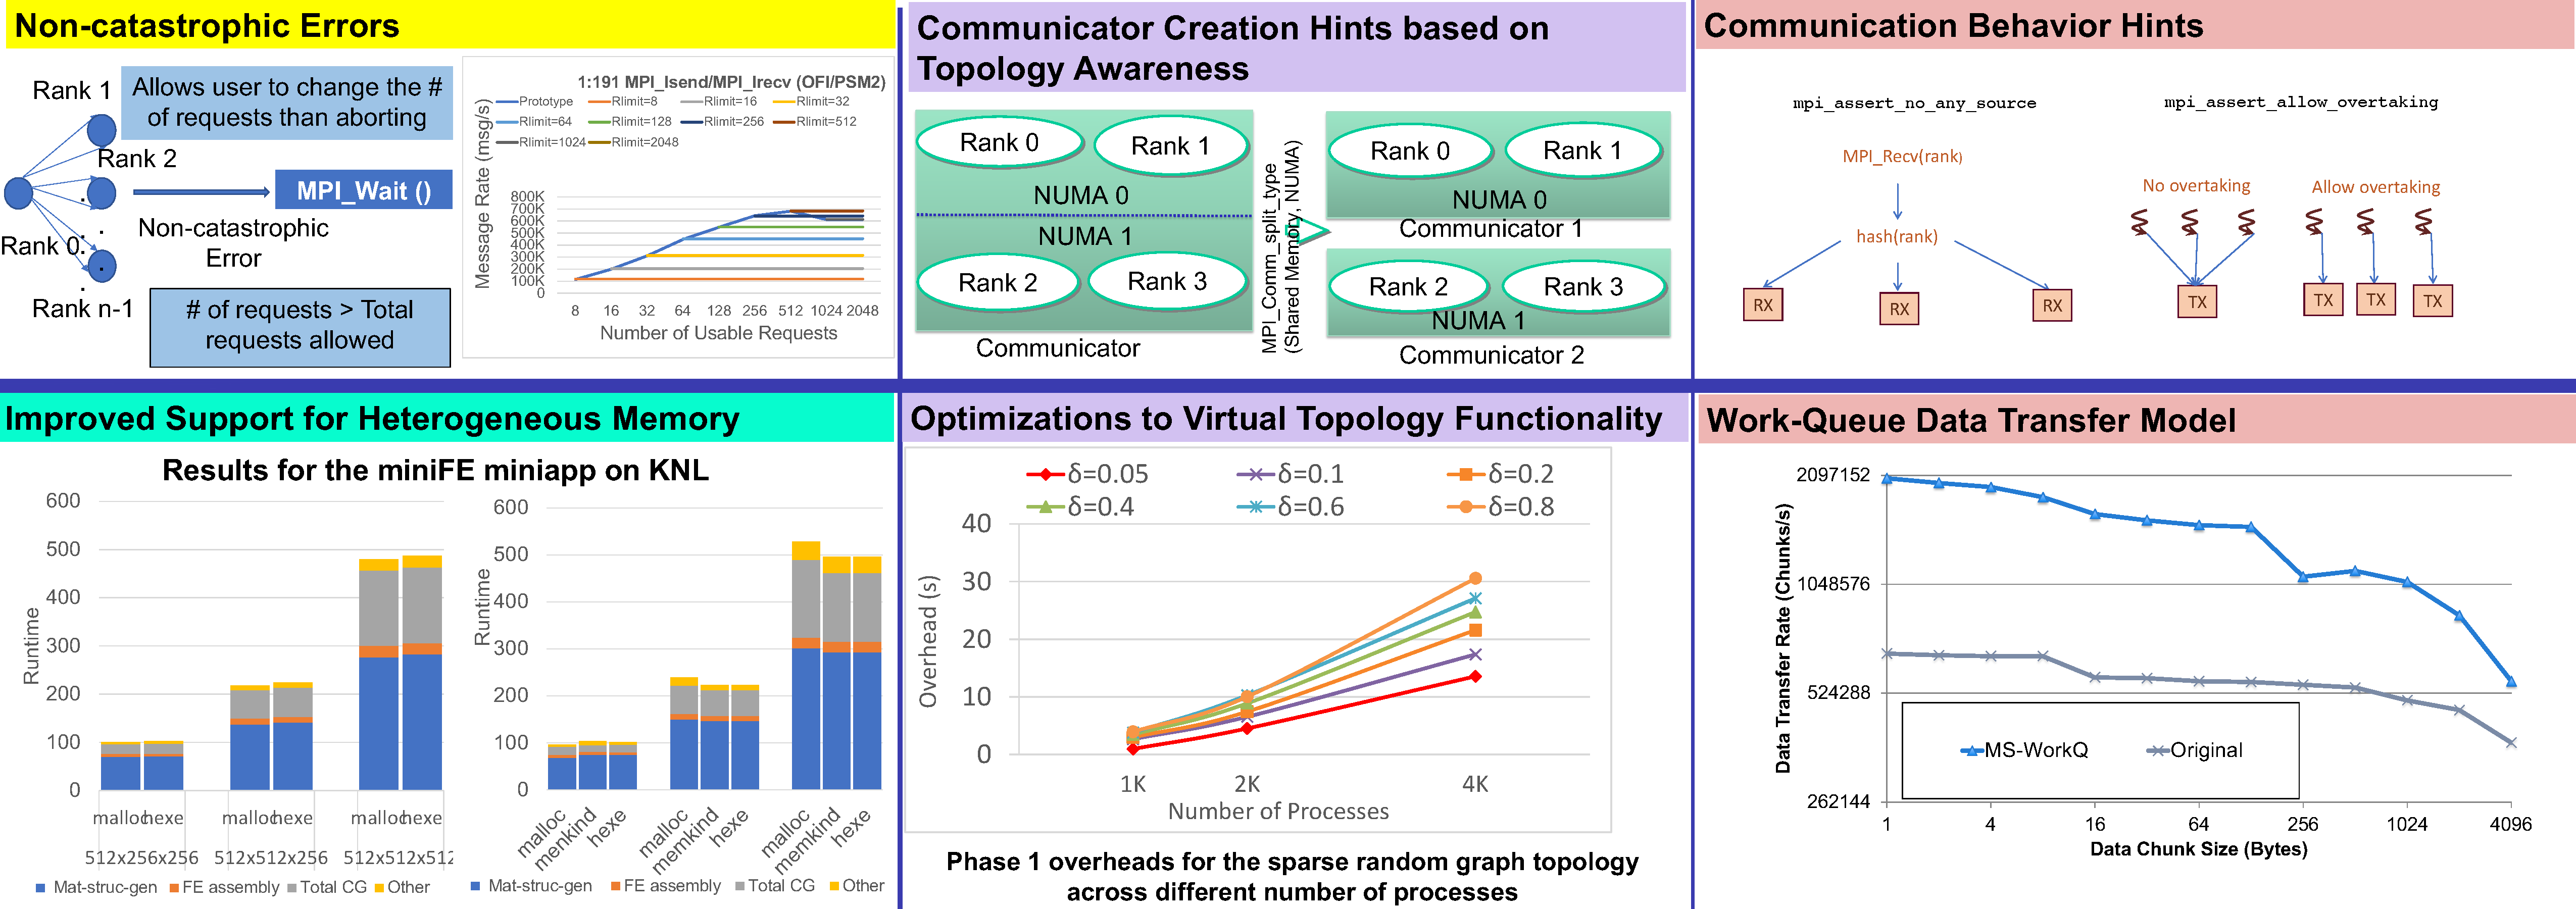
\includegraphics[width=6in]{projects/2.3.1-PMR/2.3.1.07-Exascale-MPI/MPICH-recent-milestones.pdf}
  \caption{\label{fig:march18}The details of MPICH milestones
    completed in FY18Q1 and FY18Q2}
\end{figure}

Milestones completed in March 2018 include: (1) investigating the
memory subsystem of future ECP machines to understand the possible
memory architectures; we presented and evaluated Hexe, our new
framework that improves both the flexibility and portability of memory
allocation and management of heterogeneous memory compared with other
memory allocation tools such as malloc and memkind \cite{hexe}.  (2)
designing the interface and algorithm for remapping processes and
nodes according to the topology or allocating resources based on
application communication patterns, in terms of MPI graph and
Cartesian functions.  (3) work-queues to hold work descriptors of
work-generating threads; this approach decouples work-generating
threads from completion-waiting ones and avoids interference between
them.

\paragraph{Next Steps}

Several follow-on efforts are planned for the project:

\begin{enumerate}

\item \textbf{Performance and Scalability:} Exascale MPI efforts
  include investigation and evaluation of communication relaxation
  hints, investigation of optimizations to memory scalability in MPICH
  and improvements to MPI RMA operations.
	
\item \textbf{Heterogeneity:} Exascale MPI efforts include the
  investigation of utilizing heterogeneous memory inside the MPI
  implementation and ECP application performance evaluation of
  utilizing heterogeneous memory inside the MPI implementation.
	
\item \textbf{Topology Awareness:} Exascale MPI efforts include the
  analysis of the performance evaluation of the implementation of
  virtual topology functionality, investigating topology-aware
  collectives and neighborhood collectives in MPICH and evaluate the
  selected ECP applications.
	
\item \textbf{Fault Tolerance:} Exascale MPI effort is to investigate
  for fault tolerance with the focus on evaluating applications
  suitability for ULFM in MPI, to focus on the standardization of ULFM
  in MPI and finally, investigate and evaluate the implementation of
  MPI-4 ULFM proposal in MPICH.
	
\item \textbf{MPI+X Hybrid Programming:} Exascale MPI efforts include
  the investigation and evaluation on interaction between MPI and
  OpenMP, to investigate a study of the benefit potential of the MPI
  endpoints approach and evaluate it with selected ECP applications.

\end{enumerate}
